\subsection{The end-to-end latent against its reference}
\label{sec:surrogate}
% Artifact: results/sur/surrogate_seeds/surrogate_seeds.json (3-seed GCP L4) +
% surrogate_vs_true.json via scripts/analysis/run_compensation_surrogate.py, n=44 matched VT-2005.
% Direct two-MSE cancellation check: results/compensation/two_mse_check.json via
% scripts/analysis/run_surrogate_two_mse.py (retained checkpoints only, not the three seeds).
% The coinage "compensating surrogate" was retired on 2026-08-02 with the rest of the coined
% vocabulary; the hypothesis is now named by what it says. Do not reintroduce the term.
A candidate \emph{mechanism} for the low-fidelity, end-to-end regime is this: a
$\sigma$-profile head trained \emph{end-to-end} through a fixed, misspecified closure---with no
$\sigma$ supervision in that phase---is under pressure to \emph{cancel} the closure's error rather
than to be physically faithful. The hypothesis has two parts and this section establishes only the
first. Its antecedent---that the latent leaves the reference along a direction shared across
molecules rather than as per-molecule noise---is measured. Its consequent---that the departure
cancels part of $\Bclos$---is not, and the one direct check we can run on retained checkpoints
argues against it, on the wrong axis and with little power. The external reference that fixes the
ceiling (\S\ref{sec:measure}) makes the first part testable: we compare the predicted profile
$\hat\sigma$ against the reference VT-2005 profile molecule by molecule ($n{=}44$).

\paragraph{The drift under fine-tuning.} The comparison is within a single grounded model,
checkpointed before and after solubility fine-tuning (the $\sigma$ head unfrozen), so architecture
and initialisation are held fixed and only the objective differs; it is repeated over \emph{three
seeds} and reported mean$\pm$sd. Under $\sigma$ supervision the head reproduces the reference
profile to within $36\pm1\%$, so the intermediate \emph{can} carry the physical shape, though only
as an in-sample fit: all $44$ probe molecules lie inside the $\sigma$-grounding pool
(\S\ref{sec:si-mech}). Solubility fine-tuning then drives the profile $41\pm3\%$ off the grounded
one, for a total departure from the reference of $51\pm2\%$. What this section carries is the sign
of the departure and the presence of a shared direction, not the magnitudes: that figure, and the
two below it, are not stable across analysis configurations (\S\ref{sec:si-mech}). The drift is not
per-molecule noise, and its structure is not a constant offset: the first two principal components
of the \emph{mean-centred} deviation carry $72\pm1\%$ of the variance. The quantity read against a
null is a different one, the top-two share of the learned-versus-reference deviation, $0.399$; its
null is \emph{phase-randomised}, matching each deviation's own smoothness and destroying only the
between-molecule alignment at issue, and the observed share clears it ($0.399$ against $0.221$,
$p<0.001$), at roughly $1.8\times$. The $72\pm1\%$ mean-centred share has no matched null of its
own, a wrong-molecule null built from real reference profiles does \emph{not} clear ($0.772$,
$p=1.00$), and if the case for preferring the phase-randomised null is not accepted the spectrum is
uninformative rather than supporting (\S\ref{sec:si-mech}). To test whether the structure transfers
across molecules we fit one distortion operator $D$ on half the $44$ molecules and score it on the
other half, where it predicts the drift $4.1\pm0.5\times$ better than the zero-drift (identity)
null out of sample. That null is deliberately weak, nothing controls it on these three seeds, whose
checkpoints were not retained, and a molecule-independent constant offset reaches $2.1\times$ on
the one companion run where that control can be computed, so the ratio stands against the identity
null alone; the $\pm0.5$ spans seeds at one partition, and the held-out half is homologue-saturated.
Structure \emph{beyond} an offset therefore rests on the mean-centred spectrum, not on the
ratio---and that spectrum does not exclude a shrinkage of every profile toward the corpus-mean
shape. A reference ladder calibrating the $51\%$ against uninformative baselines is in
\S\ref{sec:si-mech}; on it the drift consumes essentially all the molecular specificity grounding
had provided, as a collapse toward the corpus-mean shape would also look.

% Declared here, immediately before the paragraph that cites it, so the two-column
% float queue can place it inside this section rather than pages later.
\begin{figure}[t]
\centering
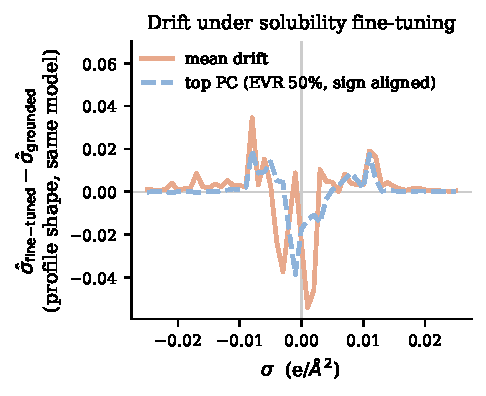
\includegraphics[width=\columnwidth]{figs/fig_compensation_surrogate.pdf}
\caption{The drift solubility fine-tuning imposes on the learned $\sigma$-profile ($n{=}44$
VT-2005-matched molecules): $\hat\sigma$ after fine-tuning minus the \emph{same model's grounded
profile}, not minus the external reference. Shown are the mean drift and its dominant PCA mode,
defined only up to sign and drawn in the mean drift's direction; the legend's EVR is that mode's
explained variance ratio.}
\label{fig:surrogate}
\end{figure}

\paragraph{Dominant mode, and the direct cancellation test.} The dominant drift mode
(Fig.~\ref{fig:surrogate}) transfers area \emph{out of} the nonpolar bins ($\sigma\!\approx\!0$)
and \emph{into} the polar wings: the network represents molecules as more polar than they are.
Whether that shift \emph{cancels} part of $\Bclos$---the input compensating the map, as the
non-identifiability of the split allows (Lemma~\ref{prop:ident})---is the comparison
$\mathrm{MSE}(m,g(\hat\sigma))$ against $\mathrm{MSE}(m,g(\zstar))$ on the same pairs. It does not
support the cancellation reading. Holding the cavity area at its reference value so that only the
profile shape varies, the sole retained end-to-end SLE-trained COSMO-SAC checkpoint gives $18.75$
against $1.47$: on the activity axis its drifted profile is an order of magnitude \emph{worse}
through the same closure, not better. Three limits sit on that number. The checkpoint is the
uncontrolled one, whose departure ($82\%$) is half again the three-seed $51\pm2\%$, so it may not
be representative of the three seeds. The axis is wrong: the drift is produced by the
finite-composition solubility objective and scored here at infinite dilution. The check also has
almost no power in the direction that matters, so it can separate ``no cancellation'' from ``large
cancellation'' but not from ``some cancellation'' (\S\ref{sec:si-mech}). It is the only direct
evidence available, and it is evidence against rather than a clean pass or fail. A second,
independent check on the closure's own axis points the same way: a \emph{more} polar profile moves
$g$ further from $m$ (\S\ref{sec:si-mech}). Both sit on that same infinite-dilution axis, so
neither refutes cancellation in the regime that generates the drift; they remove the one place it
could have been measured, and the cancellation reading remains inferred from the paradox itself. What is established is weaker and still consequential: the model's
``physical'' intermediate is not the molecule's charge distribution, consistent with cautions that
the interpretability of physics-grounded latents is not guaranteed under misspecification
\cite{brynjarsdottir2014,takeishi2021}, and that adapting a representation can itself collapse an
otherwise physically-faithful latent \cite{interno2026}. Its \emph{structure}---low-rank rather
than diffuse---excludes a random collapse but not the structured shrinkage above; the diagnostic
that would separate them is under-resolved here (\S\ref{sec:si-failed-diagnostics}).

\paragraph{What leaves $\sigma$ under-determined by activity.} The freedom that
would make such a cancellation possible is the closure's geometry: at infinite dilution the
activity map concentrates on the one or two hydrogen-bonding directions where the closure is least
faithful (\S\ref{sec:map}). The end-to-end head can therefore move $\sigma$ along the remaining,
low-sensitivity directions at little cost to the fit---the $\sigma$-profile form of
Lemma~\ref{prop:ident}. The Fisher measurement behind that statement, and the two respects in which
it does not settle the question, are in \S\ref{sec:si-mech}; nothing here shows recovery of the
physical profile to be impossible in principle. The sign of grounding turns on \emph{both} axes,
and on which sense of grounding is meant. Freezing the $\sigma$ head at its supervised warm-up
state instead of letting it drift end to end cuts the reference-input penalty by $65\%$
($\Delta\mathrm{MAE}$ from $+0.40$ to $+0.14$ over $n{=}5571$ matched test rows). Those are a
separate matched pair of runs, one base resumed twice with the freeze off and on, and not the
$+0.41$ headline arms of \S\ref{sec:paradox} (\S\ref{sec:si-tables}). A near-physical intermediate
makes the pipeline far more robust to substituting the reference $\sigma$. Supervision alone does
not, however, \emph{flip} the sign here---the penalty stays positive, the closure still being the
low-fidelity COSMO-SAC-2002 and the warm-up $\sigma$ itself only partly physical. The full flip
needs supervision \emph{and} fidelity together, which is what TeNNet-SAC \cite{yang2025tennet} has
and this pipeline does not (\S\ref{sec:intro}).
